
\documentclass[preprint,12pt]{elsarticle}

\usepackage[spanish]{babel}
\usepackage{amssymb}
\usepackage{graphicx}
\usepackage{lineno}
\usepackage[utf8]{inputenc}
\usepackage{url}
\usepackage{natbib} 
\usepackage{amsmath} 
\usepackage{amssymb} 

\begin{document}
	
	\begin{frontmatter}

		\title{\huge Las nuevas caracteristicas de un estandar ISO de SQL-1992}
		
		\author{Estrella Palacios, Katherine Lizbeth              (2016056193))}
		
		\address{Tacna, Perú}
		
		\begin{abstract}
			%% Text of abstract
SQL (structured query language), in addition to allowing us queries in the database, contains primitives for defining tables, updating the database, defining views granting privileges, etc. Aspects of the 1992 ANSI standard, known as SQL-92, are shown below.
		\end{abstract}
\end{frontmatter}
%%
	%% Start line numbering here if you want
	%%
	%\linenumbers
	
	%% main text
	\section{Resumen}

SQL (Structured Query Languaje) además de permitirnos consultas en la base de datos, contiene primitivas de definición de tablas, actualización de la base de datos, definición de vistas otorgamientos de privilegios, etc. A continuación se mostrarán aspectos del estándar ANSI de 1992, conocido como SQL-92.

%%cambiar
\section{Introducción} 
SQL-92 fue desarrollado por el comité técnico NCITS H2 sobre bases de datos. Este comité desarrolla estándares para la sintaxis y semántica de los lenguajes de bases de datos. SQL-92 fue diseñado para ser un estándar para los sistemas manejadores de bases de datos relacionales (RDBMS). Esta basado en SQL-89, cuya primera versión se conoce como SQL-86. En 1992 aparece SQL2 o SQL92, la versión hoy en día más difundida ([ISO/IEC 1992] [ANSI 1992] [ISO/IEC 1994]). Con la aparición de la segunda versión del estándar (SQL2) en 1992, prácticamente todos los RDBMS, incluso los no relacionales, incluían soporte a SQL. Hoy en día, SQL se ha convertido en el lenguaje de consulta más utilizado. Las nuevas características de SQL-92 son:
\begin{itemize}
\item Nuevos tipos de datos definidos: DATE, TIME, TIMESTAMP, INTERVAL, BIT string, VARCHAR strings, y NATIONAL CHARACTER strings.
\item Soporte adicional codificación de caracteres más allá del requisito base para representar sentencias SQL.
\item Nuevas operaciones escalares tales como concatenación de cadenas y extracción de subcadenas, matemáticas, de fecha y hora y declaraciones condicionales.
\item Nuevas operaciones como UNION JOIN, NATURAL JOIN, establecer diferencias y establecer intersecciones.
\item Expresiones condicionales con CASE.
\item Soporte alternativo para el Lenguaje de Definición de Datos (DDL por sus siglas en inglés) a través de ALTER y DROP.
\item Posibilidad de enlazar C (lenguaje de programación), Ada (lenguaje de programación) y MUMPS.
\item Nueva funcionalidad para controlar los privilegios de usuario.
\item Nueva funcionalidad de comprobación de la integridad, como la restricción de verificación.
\item Un nuevo esquema de información de sólo lectura sobre metadatos de la base de datos como, por ejemplo, las tablas que contiene, etc. 
\item Ejecución dinámica de sentecias (en luegar de prepararlas).
\item Mejor soporte para acceso remoto.
\item Tablas temporales. Por ejemplo, CREATE TEMP TABLE etc.
\item Transacciones.
\item Nuevas operaciones para cambiar tipos de datos en el momento indicado a través de CAST (expr AS type).
\item Cursores.

\end{itemize}
%% ----------------------------------------------------------------------------------------------------------------------------------
\section{Marco Teórico}
%%Aspectos Generales de SQL
\subsection {\textbf{SQL}}

\subsubsection{\textbf{Definición}}
SQL. Structured Query Language (lenguaje de consulta estructurado), es un lenguaje surgido de un proyecto de investigación de IBM para el acceso a bases de datos relacionales. Actualmente se ha convertido en un estándar de lenguaje de bases de datos, y la mayoría de los sistemas de bases de datos lo soportan, desde sistemas para ordenadores personales, hasta grandes ordenadores. \cite{SQLne}

\subsubsection{\textbf{Orígenes y evolución}}
Los orígenes del SQL están ligados a los de las bases de datos relacionales. En 1970 Codd propone el modelo relacional y asociado a este; un sublenguaje de acceso a los datos basado en el cálculo de predicados. Basándose en estas ideas los laboratorios de IBM, definen el lenguaje SEQUEL (Structured English Query Language) que más tarde sería ampliamente implementado por el SGBD experimental System R, desarrollado en 1977 también por IBM. Sin embargo, fue Oracle quien lo introdujo por primera vez en 1979 en un programa comercial. El SEQUEL terminaría siendo el predecesor de SQL, siendo éste una versión evolucionada del primero. El SQL pasa a ser el lenguaje por excelencia de los diversos SGBD relacionales surgidos en los años siguientes y es por fin estandarizado en 1986 por el ANSI, dando lugar a la primera versión estándar de este lenguaje, el SQL-86 o SQL1. 

\begin{figure}[htb]
	\begin{center}
		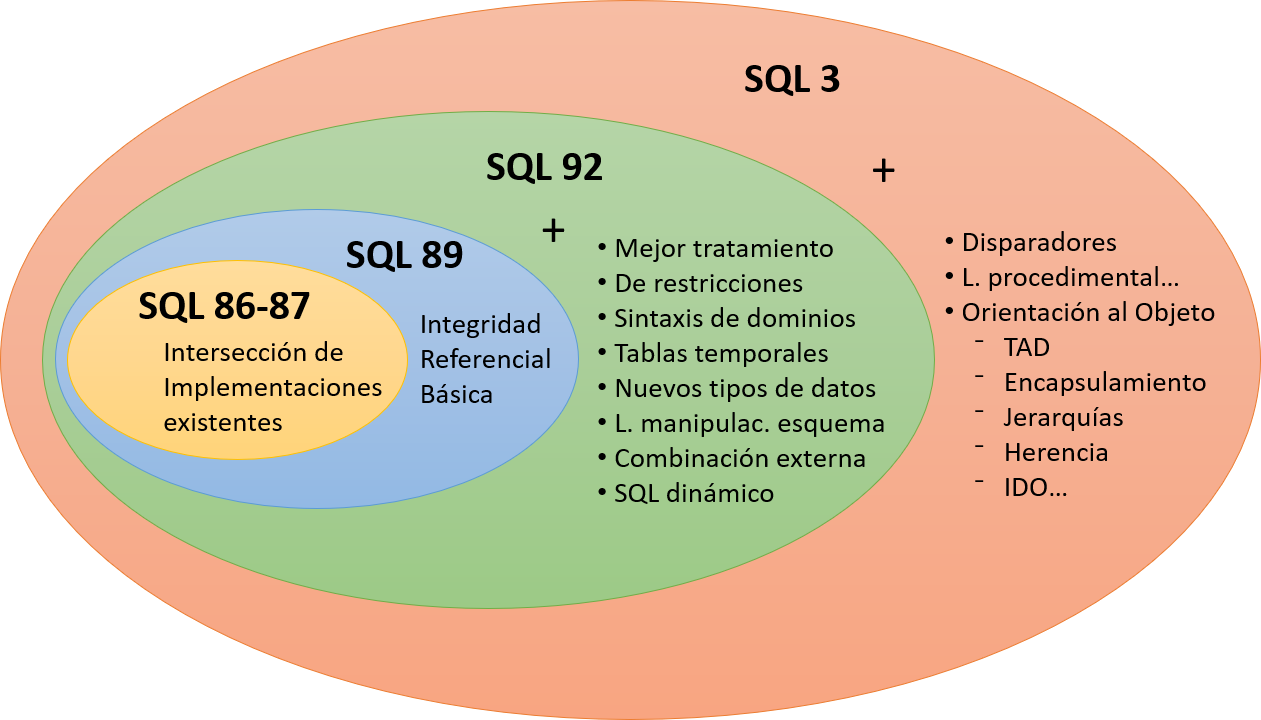
\includegraphics[width=10.5cm]{./IMAGENES/evolucion}
		%%\caption{Pie de figura}
  		%%\label{etiqueta}
	\end{center}
\end{figure}

Al año siguiente este estándar es también adoptado por la ISO. Sin embargo este primer estándar no cubre todas las necesidades de los desarrolladores e incluye funcionalidades de definición de almacenamiento que se consideraron suprimir. Así que en 1992 se lanza un nuevo estándar ampliado y revisado del SQL llamado SQL-92 o SQL2. En la actualidad el SQL es el estándar de facto de la inmensa mayoría de los SGBD comerciales. Y, aunque la diversidad de añadidos particulares que incluyen las distintas implementaciones comerciales del lenguaje es amplia, el soporte al estándar SQL-92 es general y muy amplio. \cite{SQLne}
\\ En la figura anterior se muestra la evolución del SQL-86 al SQL-3. \cite{Miguel1999}

\subsubsection{\textbf{Tipos de sentencias SQL}}
Como su nombre indica, el SQL nos permite realizar consultas a la base de datos. Pero el nombre se queda corto ya que SQL además realiza funciones de definición, control y gestión de la base de datos. Las sentencias SQL se clasifican según su finalidad dando origen a tres ‘lenguajes’ o sublenguajes:
\begin{itemize}
\item El DDL (Data Definition Language), lenguaje de definición de datos, incluye órdenes para definir, modificar o borrar las tablas en las que se almacenan los datos y de las relaciones entre estas. Es el que más varia de un sistema a otro.

\item El DCL(Data Control Language), lenguaje de control de datos, contiene elementos útiles para trabajar en un entorno multiusuario, en el que es importante la protección de los datos, la seguridad de las tablas y el establecimiento de restricciones en el acceso, así como elementos para coordinar la compartición de datos por parte de usuarios concurrentes, asegurando que no interfieren unos con otros.

\item El DML (Data Manipulation Language), lenguaje de manipulación de datos, nos permite recuperar los datos almacenados en la base de datos y también incluye órdenes para permitir al usuario actualizar la base de datos añadiendo nuevos datos, suprimiendo datos antiguos o modificando datos previamente almacenados.

\item PLSQL( SQL Programático: Define un cursor para una consulta. DECLARE: Abre un cursor para recuperar resultados de consulta OPEN Recupera una fila de resultados de consulta, FETCH, CLOSE: Cierra un cursor.)\cite{SQLne}
\end{itemize}

%% SQL-92
\subsection{\textbf{Nuevas Características de SQL-92}}

\subsubsection{\textbf{Definición de Esquemas}}

La definición de un esquema es simple. Sólo se necesita identificar el comienzo de la definición con una instrucción CREATE SCHEMA y una cláusula adicional AUTHORIZATION y a continuación definir cada dominio, tabla, vista y demás en el esquema. 

\subsubsection{\textbf{Tipos de datos y dominios}}	

Un dominio es un conjunto del cual toma sus valores una columna de una relación. Según este concepto, los tipos de datos predefinidos son dominios. Adicionalmente SQL-92 permite la definición de dominios por parte de los usuarios.

\begin{itemize}
	\item \textbf{Numéricos exactos:}
	\begin{figure}[htb]
		\begin{center}
			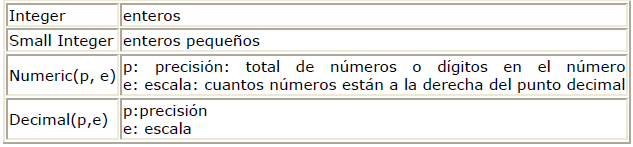
\includegraphics[width=11.5cm]{./IMAGENES/num_exactos}
		\end{center}
	\end{figure}
	
	
	\item \textbf{Numéricos aproximados:} Estos tipos de datos se utilizan normalmente para cálculos científicos y de ingeniería.
	
	\begin{figure}[htb]
		\begin{center}
			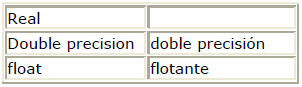
\includegraphics[width=6cm]{./IMAGENES/num_aprox}
		\end{center}
	\end{figure}
	
	
	\item \textbf{Cadenas de caracteres:} Los campos de character siempre almacenan n caracteres, aún cuando tengan que rellenar con blancos a la derecha para completar la longitud n. Los campos character varying sólo almacenan el número real de caracteres que se introdujeron (hasta un máximo de n). \\
	\begin{figure}[htb]
		\begin{center}
			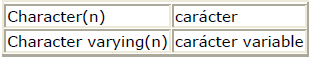
\includegraphics[width=6cm]{./IMAGENES/caracteres}
		\end{center}
	\end{figure}
	
	
	\item \textbf{Cadenas de bits:} Estos campos se usan para banderas u otras máscaras de bits para el control.\\
	\begin{figure}[htb]
		\begin{center}
			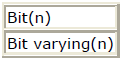
\includegraphics[width=2.5cm]{./IMAGENES/bits}
		\end{center}
	\end{figure}
	
	\item \textbf{Fechas y horas:} El tipo Date se da en el orden año, mes, día con cuatro dígitos para el año. El Time se da en horas (0 a 23), minutos, segundos y décimas de segundos. El Timestamp es la fecha más la hora.\\
	\begin{figure}[htb]
		\begin{center}
			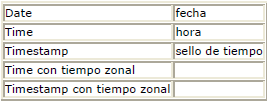
\includegraphics[width=7cm]{./IMAGENES/fechas}
		\end{center}
	\end{figure}
	
	
	\item \textbf{Intervalos:} Un intervalo es la diferencia entre dos fechas (año-mes) o entre dos horas (día-hora).\\
	
	%%\begin{figure}[htb]
		%%\begin{center}
			%%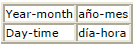
\includegraphics[width=4cm]{./IMAGENES/intervalos}
		%%\end{center}
	%%\end{figure}
\end{itemize}


\subsubsection{\textbf{Definición de dominios:}}	
Los tipos de datos con restricciones (constrains) y valores por defecto (default values) se pueden combinar en la definición de dominios. Una definición de dominio es un tipo de datos especializado que puede estar definido dentro de un esquema y utilizado en la definición de columnas. Por ejemplo:
Esta definición dice que un dominio llamado IDENTIFICADOR tiene las siguientes propiedades:
\begin{itemize}
\item 1. Su tipo de datos es numérico de cuatro dígitos.
\item 2. Su valor por defecto es 0.
\item 3. Nunca puede ser nulo.
\end{itemize}

\subsubsection{\textbf{Definición de Tablas:}}	
Las tablas se definen en tres pasos:
\begin{itemize}
\item 1. Dar el nombre de la tabla.
\item 2. Definir cada columna, posiblemente incluyendo restricciones de columna.
\item 3. Definir las restricciones de la tabla.
\end{itemize}
	\begin{figure}[htb]
		\begin{center}
			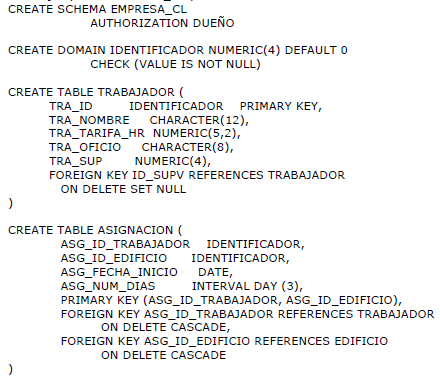
\includegraphics[width=9cm]{./IMAGENES/ejtablas}
			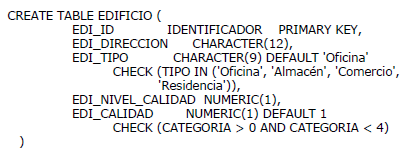
\includegraphics[width=8.5cm]{./IMAGENES/ejtablas2}
		\end{center}
	\end{figure}

Después del CREATE SCHEMA y de la definición de dominios (CREATE DOMAIN) van las instrucciones de creación de tablas. La instrucción CREATE TABLE identifica el nombre de la tabla, que debe ser única dentro del esquema. Después del CREATE TABLE van encerradas entre paréntesis y separadas por coma las instrucciones de definición de columnas y restricciones sobre la tabla. Las definiciones de columnas de la tabla (que son los atributos del modelo relacional) están compuestas por:
	\begin{figure}[htb]
		\begin{center}
			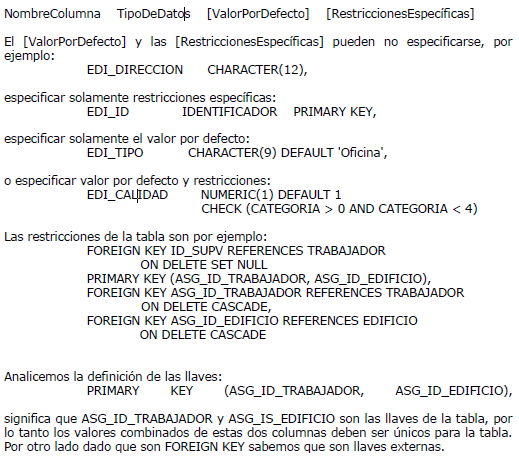
\includegraphics[width=13cm]{./IMAGENES/definiciontab1}
			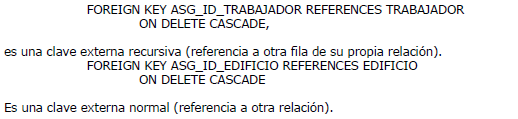
\includegraphics[width=13cm]{./IMAGENES/definiciontab2}
		\end{center}
	\end{figure}

Las palabras ON DELETE indican que hacer en caso de borrar al referido. La cláusula ON DELETE SET NULL le dice al sistema que si se borra la tupla a la que apunta la clave externa entonces el valor de ésta se debe poner a cero, esto sirve para mantener la integridad de referencias (si borro al referido, y quedan referencias apuntando a una tupla borrada tenemos una falla en la integridad de referencia). La cláusula ON DELETE CASCADE significa que si se borra la tupla referida en la relación, se realiza un borrado en "cascada" de todas las tuplas que hacían referencia a ésta. 
\\ Similar a ON DELETE tenemos a ON UPDATE y ambas cláusulas tienen las opciones siguientes:
\begin{itemize}
\item CASCADE
\item SET NULL
\item SET DEFAULT
\end{itemize}

Por último se debe decir que a diferencia de las relaciones en el modelo relaciona, no se requiere que cada tabla SQL tenga una clave primaria. En otras palabras, si no se indica ninguna clave, entonces dos filas de la tabla pueden tener valores idénticos. Lo malo es que una tabla que no tenga clave primaria no puede ser referida mediante clave externa desde otra tabla. \\ Adicionalmente SQL-92 define instrucciones para cambiar las definiciones de las tablas (ALTER TABLE) o para borrar las tablas (DROP TABLE). Para borrar un esquema completo se usa DROP SCHEMA, pero como borrar un esquema es una cosa seria, se tiene que especificar que opción de borrado se usa: \\ DROP SCHEMA NombreEsquema CASCADE: significa eliminar el esquema con ese nombre al igual que todas las tablas, datos y otros esquemas que aún existan. DROP SCHEMA NombreEsquema RESTRICT: significa eliminar el esquema sólo si todos los restantes objetos del esquema ya han sido borrados.

\subsubsection{\textbf{Manipulación de datos:}}
\begin{itemize}
%%
\item \textbf{Consultas simples:} \\ Una consulta que involucra una sola tabla de la base de datos.\\
	\begin{figure}[htb]
		\begin{center}
			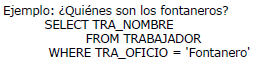
\includegraphics[width=7cm]{./IMAGENES/consultasimple}
		\end{center}
	\end{figure}
Aquí se muestran las tres cláusulas más usadas en SQL: la cláusula SELECT, la cláusula FROM y la cláusula WHERE. Una buena regla es escribir cada cláusula en una línea aparte y con sangrías, aunque se puede escribir todo en la misma línea. \\ Cláusula SELECT: Señala las columnas que se desean en la consulta (equivalente a la proyección del álgebra relacional). \\ Cláusula FROM: Lista las tablas que son referidas por la consulta. \\ Cláusula WHERE: Nos da la condición para seleccionar las filas de las tablas indicadas. \\ La sentencia SQL anterior se procesa por el sistema en el orden FROM, WHERE, SELECT. \\ Otro ejemplo: ¿Cuál es la tarifa semanal de cada electricista?, además entregue la salida ordenada alfabéticamente.
	\begin{figure}[htb]
		\begin{center}
			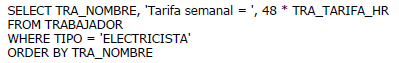
\includegraphics[width=10cm]{./IMAGENES/consultasimple2}
		\end{center}
	\end{figure}
\\ Debe notarse la inclusión de la cadena de caracteres 'Tarifa semanal = ' al cálculo de la consulta. También nótese que con la cláusula ORDER BY podemos ordenar la salida, si se quisiera orden descendente, se utilizaría "DESC". \\ Consulta: ¿Quiénes tienen una tarifa por hora entre \$ 7000 y \$ 9000, entregue toda la información de la tabla?
	\begin{figure}[htb]
		\begin{center}
			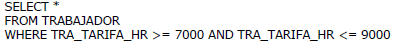
\includegraphics[width=10cm]{./IMAGENES/consultasimple3}
		\end{center}
	\end{figure}
Se pueden usar los siguientes operadores de comparación: \begin{equation*}=, <> (distinto), <, >, <=, >=\end{equation*}
\\ Se pueden usar los siguientes conectores booleanos: AND, OR, NOT. \\ \\ \\ Consulta: Indique los fontaneros, albañiles y electricistas.
	\begin{figure}[htb]
		\begin{center}
			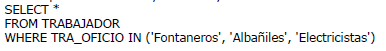
\includegraphics[width=10cm]{./IMAGENES/consultasimple4}
		\end{center}
	\end{figure}

Consulta: Encontrar todos los trabajadores cuyos oficios comiencen con "Elec". Para esto necesitamos usar caracteres comodines. Es decir, símbolos especiales que valen por cualquier cadena de caracteres.
	\begin{figure}[htb]
		\begin{center}
			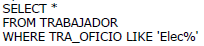
\includegraphics[width=5.5cm]{./IMAGENES/consultasimple5}
		\end{center}
	\end{figure}

SQL tiene dos caracteres comodines, el \%  que vale por cero o cualquier cantidad de caracteres, y \_ que vale por exactamente un caracter cualquiera. El operador LIKE se usa para comparar variables de caracteres literales cuando se utilizan comodines. \\ Consulta: Encuentre todas las asignaciones que comiencen en las dos próximas semanas.
	\begin{figure}[htb]
		\begin{center}
			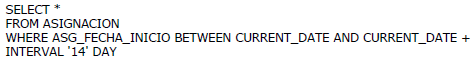
\includegraphics[width=12cm]{./IMAGENES/consultasimple6}
		\end{center}
	\end{figure}
\\ Aquí se introduce el operador BETWEEN, que devuelve VERDADERO si el valor está dentro del intervalo [CURRENT\_DAY, CURRENT\_DATE + INTERVAL '14' DAY] y FALSO si no. CURRENT\_DAY (fecha actual) es una función que siempre devuelve la fecha de hoy.\\

%%
\item \textbf{Consultas multi-tablas:} \\ Consulta: ¿Cuáles son los oficios de los trabajadores asignados al edificio 435?
	\begin{figure}[htb]
		\begin{center}
			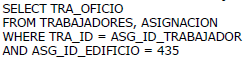
\includegraphics[width=7cm]{./IMAGENES/consultamultip1}
		\end{center}
	\end{figure}
\\En este caso, la cláusula FROM calcula el producto cartesiano de las tablas indicadas y luego con la cláusula WHERE filtramos las filas interesantes (aquellas en que TRA\_ID es igual a ASG\_ID\_TRABAJADOR) y luego las que nos interesan (las asignaciones al edificio 435), y por último SELECT toma la columna que nos interesa. Ojo que cuando hay problemas de que se repite un nombre de columna le ponemos como prefijo el nombre de la tabla seguida por un punto, ejemplo: TRABAJADORES.TRA\_ID, o ASIGNACION.ASG\_ID\_EDIFICIO. \\ Consulta: Indicar los trabajadores con los nombres de sus supervisores.
	\begin{figure}[htb]
		\begin{center}
			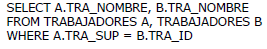
\includegraphics[width=7cm]{./IMAGENES/consultamultip2}
		\end{center}
	\end{figure}
\\En este caso, para resolver la consulta necesitamos dos copias de la tabla, para ello usamos alias (un nombre alternativo que se le da a una relación) de las tablas A y B para referirnos a cada copia.

%%
\item \textbf{Subconsultas:} \\ Una consulta dentro de una consulta.\\
Consulta: ¿Cuáles son los oficios de los trabajadores asignados al edificio 435?
	\begin{figure}[htb]
		\begin{center}
			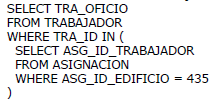
\includegraphics[width=6cm]{./IMAGENES/subconsulta1}
		\end{center}
	\end{figure}
\\ En el ejemplo la subconsulta es:
	\begin{figure}[htb]
		\begin{center}
			
\includegraphics[width=11.5cm]{./IMAGENES/subconsulta2}
			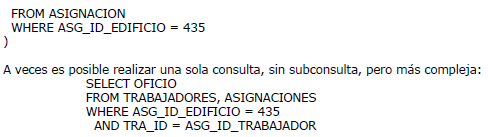
\includegraphics[width=11.5cm]{./IMAGENES/subconsulta3}
		\end{center}
	\end{figure}

\end{itemize}

\subsubsection{\textbf{Exists y Not Exists:}}
Operador EXISTS: Evalúa verdadero si el conjunto resultante es no vacío. \\ Operador NOT EXISTS: Evalúa verdadero si el conjunto resultante es vacío. \\ 
Consulta: ¿Quienes son los trabajadores que no están asignados al edificio 435?

	\begin{figure}[htb]
		\begin{center}
			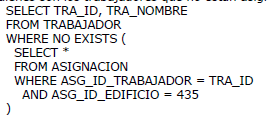
\includegraphics[width=6.5cm]{./IMAGENES/exists}
		\end{center}
	\end{figure}
Los operadores EXISTS y NOT EXISTS siempre preceden a una subconsulta.\\ Además esta subconsulta tiene apellido, es una subconsulta correlacionada, es decir, es una subconsulta cuyos resultados dependen de la fila que se está examinando por una consulta más externa.

\subsubsection{\textbf{Funciones integradas:}}
Consulta: ¿Cuáles son la tarifa por hora mayor y menor?

	\begin{figure}[htb]
		\begin{center}
			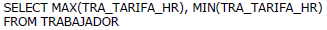
\includegraphics[width=8cm]{./IMAGENES/funintegrada1}
		\end{center}
	\end{figure}

Consulta: ¿Cuál es el promedio de días que los trabajadores están asignados al edificio
435?

	\begin{figure}[htb]
		\begin{center}
			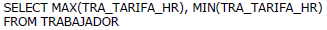
\includegraphics[width=8cm]{./IMAGENES/funintegrada1}
		\end{center}
	\end{figure}

Consulta: ¿Cuál es el número total de días asignados a fontanería en el edificio 312?

	\begin{figure}[htb]
		\begin{center}
			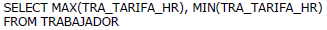
\includegraphics[width=8cm]{./IMAGENES/funintegrada1}
		\end{center}
	\end{figure}

Consulta: ¿Cuántos tipos de oficios diferentes hay?

	\begin{figure}[htb]
		\begin{center}
			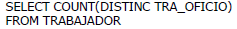
\includegraphics[width=6.5cm]{./IMAGENES/funintegrada4}
		\end{center}
	\end{figure}

La palabra clave DISTINCT se usa para que el sistema no cuente el mismo tipo de oficio mas de una vez. \\ \\Como muestran todos estos ejemplos, si una función integrada aparece en una cláusula SELECT, entonces nada más que funciones integradas pueden aparecer en dicha cláusula SELECT. La una excepción ocurre en combinación con la cláusula GROUP BY.

\subsubsection{\textbf{Group By y Having:}}
\begin{itemize}
\item Cláusula GROUP BY: Indica cuáles filas deben agruparse sobre un valor común de las columna(s) especificada(s) 
\item Cláusula HAVING: Una cláusula que impone condiciones a los grupos.
\end{itemize}
A diferencia de ORDER BY que se ejecutan sólo para ordenar la salida, GROUP BY y HAVING permiten generar particiones (grupos de datos) para realizar operaciones sobre las particiones. \\ \\Consulta: Para cada supervisor, ¿Cuál es la tarifa por horas más alta que se le paga a
un trabajador que informe a este supervisor?\\ \\ \\

	\begin{figure}[htb]
		\begin{center}
			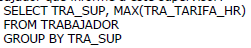
\includegraphics[width=6.5cm]{./IMAGENES/group1}
		\end{center}
	\end{figure}

Consulta: Para cada supervisor que dirige a más de un trabajador, ¿cuál es la tarifa por horas más alta que se le paga a un trabajador que informe a dicho supervisor?

	\begin{figure}[htb]
		\begin{center}
			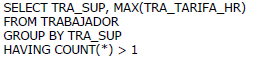
\includegraphics[width=6.5cm]{./IMAGENES/group2}
		\end{center}
	\end{figure}

Noten que la cláusula WHERE aplica a las filas, en cambio la cláusula HAVING a grupos !!, aunque pueden trabajar juntos WHERE y HAVING.\\ \\ Consulta: Para cada supervisor que dirige a más de un trabajador, ¿cuál es la tarifa por horas más alta que se le paga a un electricista que informe a dicho supervisor?

	\begin{figure}[htb]
		\begin{center}
			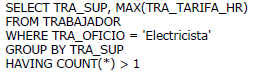
\includegraphics[width=6.5cm]{./IMAGENES/group3}
		\end{center}
	\end{figure}

\subsubsection{\textbf{Operaciones de modificación de la base de datos:}}
\begin{itemize}
\item INSERT: Operación que causa que se añadan filas a una relación.
\item UPDATE: Operación que cambia los valores de las columnas en las filas.
\item DELETE: Operación que quita filas de una relación.
\end{itemize}

A continuación podemos ver ejemplos de inserción y actualización:
	\begin{figure}[htb]
		\begin{center}
			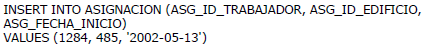
\includegraphics[width=11cm]{./IMAGENES/insert}
		\end{center}
	\end{figure}

	\begin{figure}[htb]
		\begin{center}
			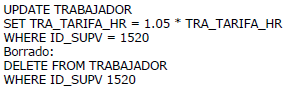
\includegraphics[width=7.5cm]{./IMAGENES/update}
		\end{center}
	\end{figure}

\subsubsection{\textbf{Definición de vistas:}}
Una vista es una porción restringida de la base de datos, y se obtiene de una tabla que contiene información básica o real. Por ejemplo si quisieramos crear una vista de la tabla TRABAJADOR pero que no muestre su tarifa por hora:

	\begin{figure}[htb]
		\begin{center}
			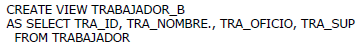
\includegraphics[width=10cm]{./IMAGENES/vistas1}
		\end{center}
	\end{figure}



%% ----------------------------------------------------------------------------------------------------------------------------------

\section{Análisis}



%% ----------------------------------------------------------------------------------------------------------------------------------

\section{Conclusiones}
\begin{itemize}
\item Conclusion 1 : \\ El lenguaje de consulta estructurado de ANSI nos permite manejar nuestra base de datos de manera rápida y confiable, con la seguridad de recibir los informes tal y como sean requerids por los usuarios.

\item Conclusion 2 : \\ Con la ayuda de los sublenguajes que contienen las distintas versiones se nos hace más práctico el uso de esta herramienta. El uso de los comando DML, que conforman la base para una preparación adecuada, en la construcción de aplicaciones con BD. Las aplicaciones manejan comandos de inset, delete, update y select, contra la base de datos.

\item Conclusion 3 : \\ Finalmente, podemos concluir que SQL es un lenguaje que ha ido variando y mejorando su rendimiento con el tiempo, por lo que seguirá siendo una herramienta eficiente para el manejo de la base de datos.



\end{itemize}
%%
	
	%%
	%\linenumbers
	
	%% main text

%% ----------------------------------------------------------------------------------------------------------------------------------	
	\newpage
	
	\bibliographystyle{apalike} 	%ESTILO
	\bibliography{BIBLIOGRAFIA}	 

%% https://www.iso.org/standard/63555.html
%% https://books.google.com.pe/books?id=ILJJDwAAQBAJ&pg=PT123&dq=SQL:2016+is+the+ISO/IEC+9075:2016+standard+of+2016&hl=es&sa=X&ved=0ahUKEwjJlKLIlYbkAhVxoFkKHc6NADMQ6AEIJzAA#v=onepage&q=SQL%3A2016%20is%20the%20ISO%2FIEC%209075%3A2016%20standard%20of%202016&f=false
%% http://www.coninteres.es/sql/material/Estandares_ANSI-SQL.pdf
%% https://es.scribd.com/presentation/272788224/Evolucion-Ansi-SQL

	
%ARCHIVO .bib
	
	%% The Appendices part is started with the command \appendix;
	%% appendix sections are then done as normal sections
	%% \appendix
	
	%% \section{}
	%% \label{}
	
	%% References
	%%
	%% Following citation commands can be used in the body text:
	%% Usage of \cite is as follows:
	%%   \cite{key}          ==>>  [#]
	%%   \cite[chap. 2]{key} ==>>  [#, chap. 2]
	%%   \citet{key}         ==>>  Author [#]
	
	%% References with bibTeX database:
	
	
	%% Authors are advised to submit their bibtex database files. They are
	%% requested to list a bibtex style file in the manuscript if they do
	%% not want to use model1-num-names.bst.
	
	%% References without bibTeX database:
	
	% \begin{thebibliography}{00}
	
	%% \bibitem must have the following form:
	%%   \bibitem{key}...
	%%
	
	% \bibitem{}
	
	% \end{thebibliography}
	
\end{document}

%%
%% End of file `elsarticle-template-1-num.tex'.
